% !TEX root = ../thesis_main.tex
\chapter{Materials and methods}\label{chap:MaterialsAndMethods}
    \section{Parahydrogen generation and quantification}
    Parahydrogen was generated using a coldhead surrounding a chamber of $\mathrm{FeO_4}$ catalyst which was built before the beginning of this work. The setup is positioned on top of the laboratory building's roof for security reasons with the coldhead on the outside and the temperature sensitive equipment on the insisde. Holes were drilled to make the connections for vaccum hoses, sensor cables and pump exhaust.
    \begin{figure}
        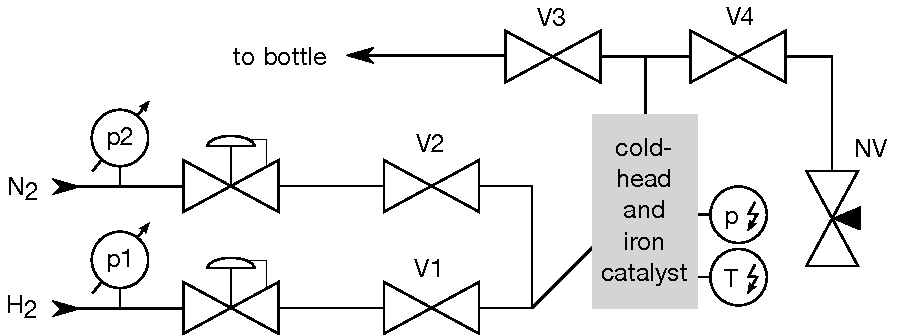
\includegraphics[width=0.99\textwidth]{/figures/materialsMethods/setupParahydrogenGenerator.pdf}
        \caption[Parahydrogen generator scheme]{The schematics of the parahydrogen generator's valve system used for reproducible and continuous production of pH2. In the lower left, the two gases, H2 and N2 are inserted into the system at defined pressures. After flowing through the central part, the coldhead, the flow against ambient pressure can be set via the needle valve before redirecting it towards the bottle to be filled.}
        \label{figure:materialsMethods:pH2Generator}
    \end{figure}
        \subsection{Coldhead side}
            The coldhead was cooled down to \SI{21}{\kelvin} via a watercooled helium recondenser with a closed helium circuit. The recondenser was operated at full power while a heater was installed to keep temperatures at 21 K. The coldhead was isolated from surrounding warm air by a vacuum chamber pumped down by a rotary vane pump. A sensor attached to the vaccum chamber read pressures to ensure sufficient isolation before switching on the recondenser. Temperature sensors in the catalyst chamber and on top of the coolant line were used for checking whether the conversion can be started and also as a feedback for the heater to regulate temperature.
        \subsection{Hydrogen side}
            The system was usually flooded with nitrogen gas before use to ensure that no explosive mixtures could built. As the nitrogen freezing point is at \SI{}{\kelvin}, it needed to be removed before cooling though. This was done by flushing the system with hydrogen gas. The system consisted of the hydrogen and nitrogen supply bottles (\SI{10}{\liter}, \SI{200}{\bar}, 99.999\% pure), both with individual pressure regulators and additional cutoff valves. The lines from the supply bottles then combine into a single line running towards and trough the coldhead and its catalyst chamber where the conversion occurs. Behind that coldhead, a needle valve regulates flow and can be switched between a flow meter to measure and set the flow against atmospheric pressure and a bottle storing the parahydrogen. Pressure limits given by the manufacturer are \SI{50}{\bar}. 
        \subsection{Parahydrogen quantification}
            To quantify the parahydrogen fraction of the gas bottled at the generator, fast NMR sequences of the gas were recorded. To do so, it was filled into a laboraty glass tube that was thoroughly cleaned and put into a 1H quad coil. The measured spectrum was compared to a nitrogen sample inside the same tube to subtract background signal from tube and plug. Additionally, a spectrum of thermal hydrogen was recorded off which the parahydrogen content is known. The parahydrogen fraction was calculated as follows: \todo{rewrite corretly}
            \begin{equation}
                f_{pH2} = \frac{S_{xx}-S_{N2}}{S_{H2}-S_{N2}} = \frac{xx}{\tfrac{3}{4}} = \frac{3}{4} \cdot xx
            \end{equation}
        \subsection{Parahydrogen decay}
            To monitor the lifetime of parahydrogen, the quantification method was used multiple times over the course of days. The decrease in parahydrogen fraction could be monitored and may be different for different means of storage, i.e. in our case, different bottles.
        \section{Low field Spectrometer}
        To acquire NMR spectra at fields where 1H-Sabre is feasible \todo{Ref sabre}, a low field NMR spectrometer was built \todo{ref niels} previous to this work as shown in figure \ref{figure:materialsMethods:lowFieldSpec}. Its main field is generated by a resisitve coil in solenoid or dual helmholtz assembly design. Inside that coil, there is a saddle coil generating a $B_1$ field perpendicular to $B_0$. Inside and perpendicular to both, a third coil, usually a solenoid, is used to detect the signal generated through the spin manipulation. The saddle coils are aligned in a way that they show axis symmetry around the rotational axis of the tube theyre mounted onto.The dimensions were chosen to fit the ratio mentioned in the theory section, (\ref{theorySaddleCoils}), i.e. \SI{35}{\cm} by \SI{80}{\cm} \todo{dims}. All coils are interchangable for others, e.g. the B0 coil can easily be exchanged for another one if a mors sophisticated design is found. Also differently sized samples or different nuclei can be measured by interchanging the receive coil.
        \begin{figure}
            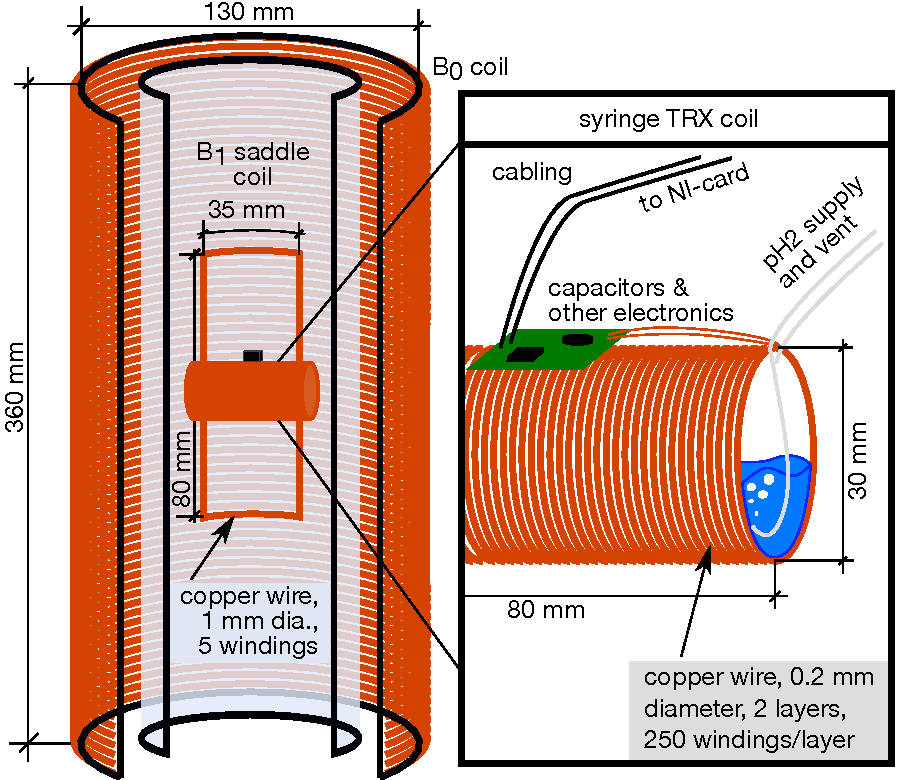
\includegraphics[width=0.99\textwidth]{/figures/materialsMethods/lowFieldSpectrometer/spectrometer.pdf}
            \caption[Schematic view low field spectrometer]{A cut view of the low field spectrometer used in the experiments. Note that only one of the two saddle coils is displayed, the other is exactly opposite of the first with the current sprouducing a field pointing in the same direction.}
            \label{figure:materialsMethods:lowFieldSpec}
        \end{figure}
        \subsection{Static magnetic field}
            Multiple coil designs of the static field generating coils have been  considered, simulated, built and tested in the course of this work. The previously used solenoid design with different lengths of compensation windings \ref{simulation:B0} showed to have disadvantages over the dual helmholz asssembly built during this work.
        \subsubsection{Solenoid coil}
            The $B_0$ coil is wound around an acrylic tube in two full layers. In addition, at the
            tube's ends, compensation windings are installed to homogenize the field inside the coil.
            The length of these windings was optimized in matlab simulations \ref{} \todo{figure of whole setup}
            Coils ususally consist of one or more layers of wire usually wound around a PVC tube. Spacing between layers is given by wire thickness including insulation coating. To keep  these distances small and, in turn, current- and thus magnetic flux density high, enameled wire was used for all coils. Winding of the wire was mostly performed on a turning lathe enabling automatic counting of the number of windings and a steady, cosistent feed of the wire.
            The solenoid coil used in the main low field experiments consisted of a three layered solenoid with two layers of compensation windings on each side. The main layers consisted of NN windings with an inner diameter of \SI{130}{\mm}. The overall length is \SI{350}{\milli\meter}. The length of the compensation windings was \ref{} \SI{}{\mm}
            \begin{figure}
                \centering
                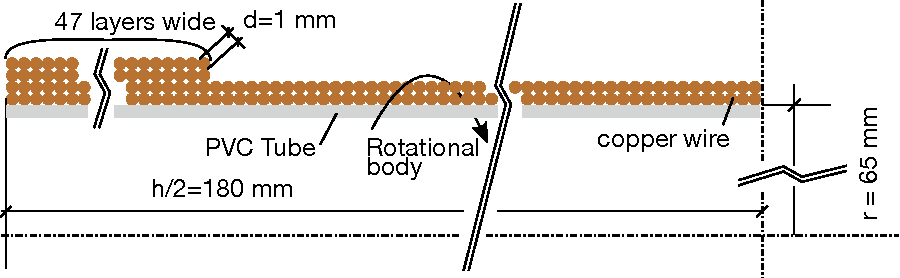
\includegraphics[width=0.99\textwidth]{/figures/materialsMethods/lowFieldSpectrometer/B0Solenoid.pdf}
                \caption[B0 coil layout]{Dimensions and structure of the standard coil used in the low field experiments to generate a homogeneous field. Note te two additional layers of wiring on the left that act as a field homogenization device.}
            \end{figure}
        \subsubsection{Helmholtz coil}
            As in the solenoid case, before building the dual helmholtz array, simulations were performed.  As space was limited inside the Mu metal shield the coil was also supposed to be used in, the coils' diameters were predetermined and only the coils distances and currents were optimized (see \ref{simulations:B0} for details). As the general setup, a PVC tube onto which four coil holders were mounted was chosen. Using the simulation results, a layout for the coil holders was designed. To keep unwanted fields due to connecting wires to a minimum, these wires were kept as short as possible. Holders were lathed and then processed further by hand. Winding of the wire was also done by hand. To keep the wire form sliding into the gouges of the previous layer, PVC foil was lasercut to fit the dimensions of the coil holders. Due to the limited size of the foil used (Din A4) and the relatively large diameter of the coils, three stripes of foil were connected with one of the three parts employing a feedthrough for the wire transversing from one layer to the next. 
        \subsection{Radiofrequency excitation}
            To irradiate samples with radiofrequency pulses, a rounded saddle coil of \SI{200}{\mm} length and \SI{100}{\mm} width was used. The manufacturing process consisted of winding the coil inside a wire holder at first. The holder was a rectangular, two parted slitted aluminum plate. The wire was wound into the slit and formed a stacked design. Then the wire layers were glued together to construct a solid connection between them.  Finally, the assembly is bent into shape using a smaller diameter PVC tube that after relaxation, the radius compares to that of the larger PVC tube. The coil was operated untuned and unmatched as a broadband resonator. The pulse generation was performed using a National Instruments data acquisition crate (NI DAQ ) which's signal was amplyfied with an audio amplifier (Onkyo ).
            The pulse was constructed using the hypercontrol software described later (\ref{}). Generally, block pulses were used but arbitrary pulseforms are possible with the card as long as the contained frequencies are below \SI{500}{\kilo\hertz} (Nyquist-Shannon). 
            \begin{figure}
                \centering
                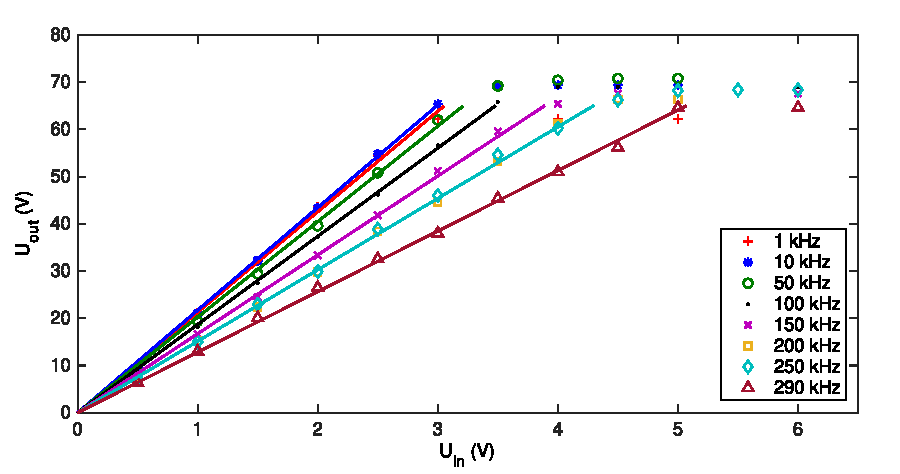
\includegraphics[width=0.99\textwidth]{/figures/materialsMethods/lowFieldSpectrometer/amplifierResponse.pdf}
                \caption[Amplifier response]{The response of the Onkyo audio amplifier at different frequencies as used in the low field spectrometer. Note the saturation at input voltages above 3 to 5 \si{\volt}. Also note that for higher frequencies, the cutoff output voltage is lower than that for lower frequencies, as the amplifier was designed for frequencies below \SI{150}{\kilo\hertz}. }
            \end{figure}

        \subsection{Receive coil}
        For signal reception, multiple coils of different resonance frequencies were built for use at different fields and for different purposes. The two most used coild in the low field spectrometer were a larger diameter coil used in field homogeniety testing and for 13C experiments and a coil wound around a syringe that also featured tubing for hydrogen in- and outlet in hyperpolarizatoin experiments. The diameter of the sirynge, and thus the coils diameter was \SI{3}{\cm}, the total volume was \SI{20}{\milli\liter}. It consisted of two layer of \SI{0.5}{\milli\meter} copper wire wound around the syringe in close packing. A \ref{how big} \SI{100}{\nano\farad} capacitor was soldered to the wire endings of the coil formed that way. 
        Receive surcuits were ususally kept simple and were tuned once and then kept at that frequency, so no adjustable capacitors were used. Also, no matchning was performed as it was very difficult to perform and improvements weren't observable. The dual resonant circuits consisted of a second resonant circuit in parallel to the first.
        \subsection{Geometric decoupling}
            \begin{equation}
            \mathrm{G}=\frac{\mathrm{U_{out}}}{\mathrm{U_{rec}}(\phi)}
            \end{equation}
            where $\mathrm{U_{out}}$ and $\mathrm{U_{rec}}$ are the transmitted and received voltages and $\phi$ is the angle between the two coils.
        \subsection{Flip angle calibration}
            Flip angles were calibrated by stepping through different excitation voltages one at a time, leaving the length of the excitation pulse unchanged. The resulting signals were fitted using a matlab tool previously written in the group or a python tool written in the course of this work. Both tools fit a lorentian distribution to the data.
            The resulting data was fitted with a sinusoidal of the form
            \begin{equation}
                \mathrm{S}(\mathrm{U_{exc}})= a \cdot \sin(b\cdot \mathrm{U} + c)
            \end{equation}
            and the voltage for a  \SI{90}{\degree} angle was found from the fitted parameters:
            \begin{equation}
                \mathrm{U}_{90} = (\frac{\pi}{2}-c)/b
            \end{equation}
            The \SI{180}{\degree} pulse was double that, accordingly.
        \subsection{Fitting tools}
            To evaluate the recorded data, often, the signal area was relevant. It was calculated using one of the two programs mentioned below. To eliminate the rf-pulse and its ringdown that was usually included in the recording, a scecific number of samples, usually in the range of 2000, was dropped from the beginning of the dataset. A preimplemented FFT algorithm was used to generate the spectral representation of the data.
            \subsubsection{Matlab tool}
            The tool named 'FIT\_gui' is a matlab based program that loads data in the '.m' format and fits a lorentian to the data whose averages can either be summed over or fitted individually. Parameters adapted during fit are amplitude, width, center frequency and phase. Signal area A is calculated using full width at half maximum FWHM and amplitude a:
            \begin{equation}
                A=a\cdot\frac{FWHM\pi}{2}
            \end{equation}
            \subsubsection{Python fitting tool}
            The python tool was written with a more modular, object oriented concept in mind. Fitting functions can be arbitrarily added and fitting is a lot faster due to some fitting limitations e.g. frequency bounds. The function implemented for spectra is a Lorentzian distribution of the form
            \begin{equation}
                f(x,x_0, \gamma) = \frac{1}{\pi\gamma}\left(\frac{\gamma^2}{(x-x_0)^2+\gamma^2}\right)
            \end{equation}
            where $x_0$ is the center frequency and $\gamma$ is half width at half maximum.
            Phase has been excluded from the fitting (but can easily be added) as mostly, a manual phasing is advantageous especially for low SNR data. The fit results can be saved in an ascii file simplifying further calculations or plotting.
            The modular layout allows for reading of other filetypes as well such as bruker spectra or plain text files.
            Figures can easily be saved or modified for convenient use in publications or theses.
        \subsection{Software control}
            All software control was realized using Matlab in combination with the DAQmx libraries. The 'hypercontrol' program is previously existing code but was strongly modified in the course of this work to implement more features and fix buggy behaviour. Background execution of channel tasks has been added to enable execution of e.g. valve switching during excitation pulses. An automated shimming tool was added that searches for minima in the individual shim directions. For performance reasons, the parameter evaluated was not the area of a fit, but the interpolated frequency-difference of the points above and below half of the maximum value $f(p_{max})$: $p_l$ \& $p_{l+1}$ and $p_h$ \& $p_{h-1}$:
            \begin{equation}
                \frac{f(p_{l+1})-f(p_l)}{p_{l+1} - p_l}-\frac{f(p_{h-1})-f(p_h)}{p_{h-1} - p_l}
            \end{equation}
            Additionally, some pulse programs were implemented to automate e.g. flip angle calibration.
        \subsection{Data Readout}
            All readout was done using a 12 bit NI \todo{name} card operating 1 MS/s. The signal was recorded directly without preamplification or mixing. Not using any preamplifiers required small distances between readout coil and NI card to keep signal losses at bay. Readout rates maximum is 1.25 MS/s using only a single analog channel, but in multichannel mode which is required as signal generation is realized using the same card, 1 MS/s. This covers four points per sine for a \SI{250}{\kilo\hertz} signal and fulfils the Nyquist-Shannon-theorem. Readout bandwiths were in the range of \todo{bw} sampling \SI{1e5}{\per\second} points per acquisition, i.e. an acquisition time of \SI{0.1}{\second}.
        \subsection{Shim System}
        For homogenization of the field, a shim system was built according to Biot Savart simulations \ref{Feng}. It features linear shim coils for all three spatial dimensions mounted to a \todo{cm} acrylic tube. The x and y shims are made of four saddle coils respectively that were manufactured individually in the same way described in section \ref{} for the rf excitation coil and bent to fit the PVC tube's radius they're mounted onto. The z shims, which are basically a pair of maxwell coils, were added on top of these saddle coils. All shims were made from \SI{1}{\mm} annealed copper wire. Thick plastic foil padding of the thickness of the wire (or twice that, depending on the position) was used to keep the diameter of the second and third layer constant. All shims are driven by a \todo{H\&U} programmable power supply providing up to $\SI{10}{\ampere}$ of current per channel on four available channels. Polarity can be switched through a series of relays that are controlled via the digital outputs of the NI card. The power supply is connected via a virtual serial port inside a USB connection. That way, the three shim channels can be controlled from inside the Matlab hypercontrol program completely including switches in polarity making shimming completly automatable. \ref{subsec:hypercontrol}.
        The minimum current that can be set in constant current mode was \SI{0.1}{\milli\ampere}
        \subsection{Samples and sample preparation}
        All samples were prepared in our histology laboratory. The catalyst and solid substrates such as nicotinamide were weighed in using a microscale (). Common catalyst masses were \SI{3}{\milli\gram} to \SI{6}{\milli\gram}. The ratio of catalyst to substrate was about \SI{1/20}{} usually. The fluid substrates such as pyridine were measured using eppendorf pipettes. Same goes for the solvents.
        For activation of the solution, different methods were used: In the low field spectrometer, bubbling inside the syringe coil was one option. Another option was pre-activation inside a NMR pressure tube (\ref{}) and transfer into the syringe coil after activation. Same holds for the Magritek low field MRI system and its measurement tubes.
        In the shuttling setup \ref{}, usually the low field bubbling reactor was also used for activation. Here, the two methods previously used, bubbling and provision of high pressure, were combined for a more efficient and thus faster activation. That way, the activation time could be reduced to 20 minutes.
        Activation was confirmed by visual inspection. A yellow tint of the solution was removed after addition of hydrogen, i.e. as the solution was translucent, it was considered activated.
    \section{Magritek Low Field MRI}
            To acquire images at low fields, a Magritek Terranova \todo{ref } was used. It features similar hardware as the low field spectrometer, but uses its $B_0$ coil only for prepolarization while signal is acquired at Earth magnetic field.
        \subsection{Hardware}
            The device consists of a prepolarization coil, a shim system, an rf-excitation coil and a readout coil. All are driven by the hardware delivered by the system. An easy to use software is included with the delivery. Images and spectra were acquired with that software exclusively.
        \subsection{Imaging sequence}
        The sequence used for imaging was a standard gradient echo sequence (\ref{}).A single slice was recorded in \SI{5}{\minute} \SI{20}{\second}. Resolution was 64 x 64 with a field of view of \SI{10}{\cm}x\SI{10}{\cm} which resulted in a (\SI{1.6}{\mm})$^2$. The echo time $\mathrm{T_E}$ was set to \SI{150}{\milli\second}. The two imaged tubes contained \SI{20}{\milli\liter} H2O and the sample solution respectively. The latter consisted of \SI{6.7}{\micro\mole} IrIMes and \SI{0.3}{\milli\mole} nicotinamide dissolved in \SI{5}{\milli\liter} $\mathrm{D_20}$. The tubes had a length of \SI{100}{\milli\meter} and an inner diameter of \SI{24}{\milli\meter}. The prepolarization coil was switched on for \SI{5}{\second} before each phase encoding step generating a prepolarization field of \SI{5}{\milli\tesla} during that time. 
        %\subsection{
    \section{Bruker Low Field MRI}
        \subsection{Gradient Coil Setup}
        \subsection{Signal mixer}
        \subsection{Receive coil}
        \subsection{Paravision and Topspin software}
    \section{High field MRI}
        The most well known application of NMR is the high field MRI of human antomy with its widespread use in clinics around the world. Not as common, but equally important are preclinical scanners for research purposes. These preclinical scanner, primarily built for animal experiments, were used in most of the high field experiments shown in this work.  \subsection{MRI hardware}
            For the acquisition of spectra and images, hardware for different purposes is required:
            \begin{itemize}
            \item $B_0$ field generation
            \item Pulse generation
            \item Field gradients generation
            \item Signal readout
            \end{itemize}
            In this case, both a Bruker \SI{7}{\tesla} and a \SI{9.4}{\tesla} small animal scanner with a wide bore were used for imaging. The main magnetic field B0 is generated by a helium cooled superconductor. All hardware except for receive or TRX coils was supplied by the manufacturer, e.g. pulse generator, rf amplifier, gradient amplifiers and data aquisition crate. The trx coil used for 15N frequencies was built manually on site as there was no commercially available coil in the groups posession (see section \ref{}).
        \subsection{Gradient coil}
            The gradients used inside the imagers were BGA20 and BGA12. Both provided slew rates and gradient strengths (i.e. resolutions) that were far above what was necessary for the imaging of the phantoms shown here. Thus gradients did not pose a limitation.
        \subsection{Paravision Software}
            The standard Bruker imaging software called paravision features sequence and method implementations for the more common use cases and can additionally be modified for specific purposes. Sequence programming is generally in C++ while many other modifications can be done via GUIs.  For the purposes of this work, the most common sequences were rather simplistic NMR sequences while some images of hyperpolarized tracers have been generated with more sophisticated imaging sequences. Paravision (PV) version 5.1 was used throughout the 15N measurements as averaging during shimming is available in that version, but not in the newer PV 6.0.1.
        \subsection{Custom High Field Coils}
            Most commercially available coils are for proton imaging and spectroscopy. Coils for other nuclei are obtainable, but usually expensive and not necessarily tailored to the specific purpose in mind. Therefore, we built single and dual channel coils for different nuclei and different fields.
            \subsubsection{$\mathbf{^{15} N}$ coil}
                A solenoid of thick, stable copper wire was wound to fit the experimental setup of the shuttling system described in \ref{sec:shuttlingSystem}. The solenoid was attached to a circuit board via clamped and soldered connections. On the board, a high voltage tune capacitor as well as two symmetric matching capacitors were installed. Coaxial cable was used to make the connection to the scanner and the whole setup was mounted to a teflon holder for precise positioning.  The tune capacitor was chosen so that it can be tuned to both a $\SI{7}{\tesla}$ and a $\SI{9.4}{\tesla}$ field at $\SI{300}{\MHz}$ and $\SI{400}{\MHz}$ respectively.  \todo{image coil}
            \subsubsection{1H saddle coil} 
            An additional 1H coil for measuring fluid levels has been built. It was etched onto a single piece of copper foil and fits in between the 15N coil and the reactor. It was not used in the experiments, but can facilitate both spectroscopy and imaging of the sample. The former can be used for an overall measurement of thermal 1H sample signal and thus provide an estimate of the filling level and its development. The latter can even provide detailed insight into the actual filling levels and distribution of fluid or its position and angle in the scanner by running standard imaging sequences.
    \section{Shuttling system}\label{sec:shuttlingSystem}
    To measure in-situ Sabre polarized substances at high fields, a transfer system is necessary. This system can either move a probe inside a closed container \ref{setupNovosibirsk} or transfer the probe itself via tubings. We chose the latter for the more flexible and less difficult positioning especially in the environment of a lying bore small animal scanner as compared to a standing bore spectrometer. In addition, all actuation can be done by non-magnetic gases which was beneficial especially at the $\SI{9.4}{\tesla}$ machine which is unshielded and creates $\SI{5}{\gauss}$ fields in a distance of about $\SI{1}{\meter}$ from the scanner bore. Figure \ref{figure:materialsMethods:shields15N} shows a schematic drawing of the setup. The positioning of all the components is very flexible, i.e. every component can be placed at an individual height in z-direction. Note though that changes to one position may influence other positions, i.e. positioning is not completely uncoupled. Nevertheless, by design, the components can be aligned so that the reactor is in the most homogenous part of the B0 coil and the shims are show their most linear behavior in the same section.
        \begin{figure}
            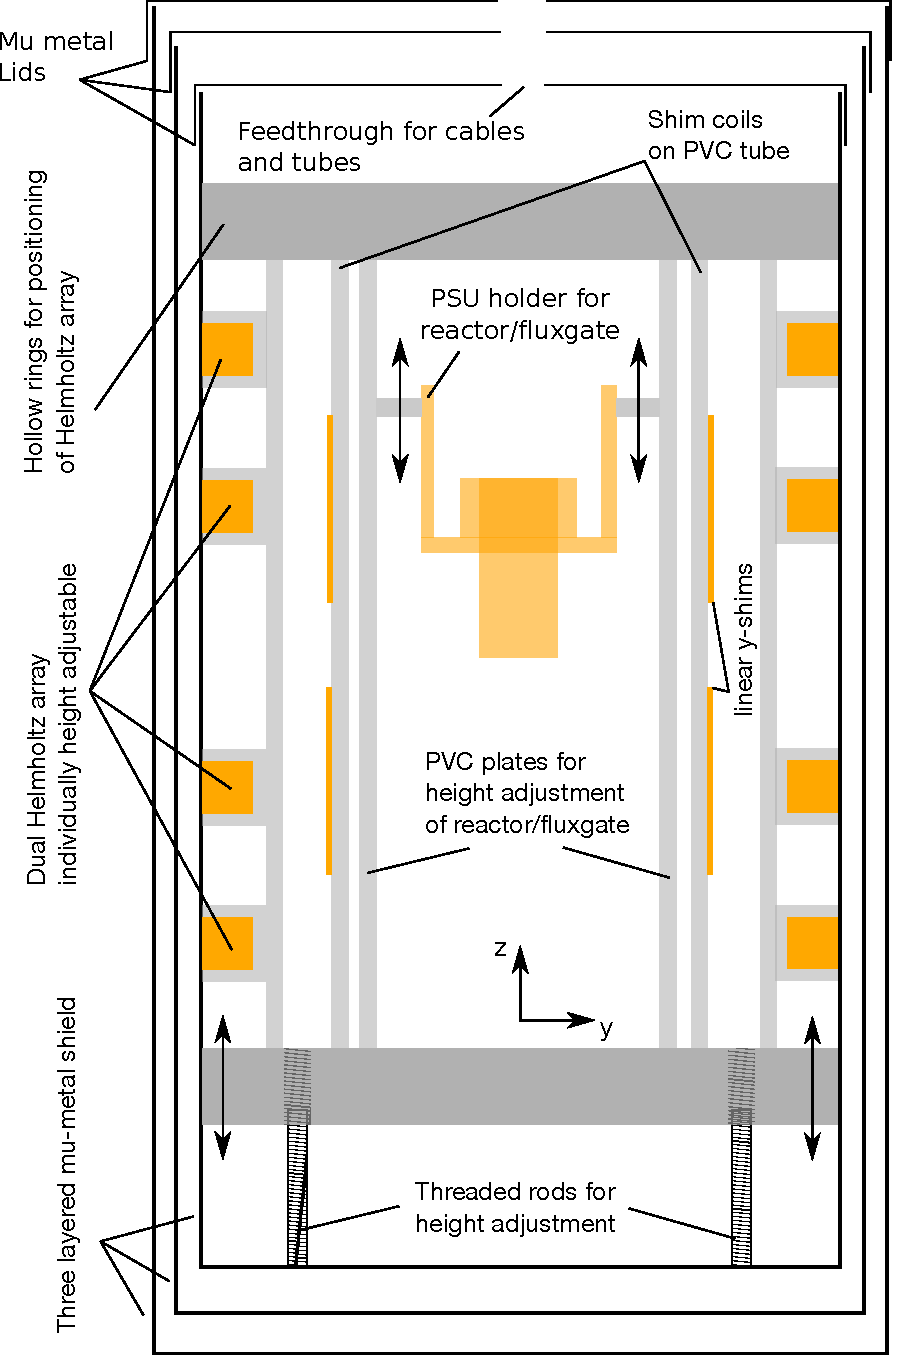
\includegraphics[width=0.99\textwidth]{/figures/materialsMethods/15NSetup/setupShield.pdf}
            \caption[Shuttling system shields]{adsf}
            \label{figure:materialsMethods:shields15N}
        \end{figure}
        \subsection{Magnetic Shielding}
        To be able to polarize $^{15}\mathrm{N}$ using Sabre Sheath \ref{}, fields of the order of
            magnitude of $\SI{100}{\nano\tesla}$ were necessary. Thus, Earth magnetic field needed to
            be shielded against. To do so, we purchased a three-layered Mu-Metal shield (ZG-218, Magnetic
            Shield Corp.) with shielding factors of 100 per layer. The dimensions of the shield are given in table \ref{table:matMeth:muMetalDims}
            \begin{table}
                \centering
                \begin{tabular}{cccc}
                    Shield No. & 1 & 2 & 3 \\
                    inner diameter & & & \\
                    outer diameter & & & \\
                    height & & &\\
                    wall thickness &\SI{1.57}{\mm}&\SI{1.57}{\mm}&\SI{1.57}{\mm} 
                \end{tabular}
                \caption[shield dimensions]{dimensions of the three layers of the mu metal shield used in the setup. note that the shields  fit into each other with a gap of about \SI{1}{\cm} in between them.}
                \label{table:matMeth:muMetalDims}
            \end{table}
            The top caps overlap the main body by \SI{30}{\mm}.  Each cap features a central hole of \SI{25}{\mm} diameter as a feedthrough for cables and tubing. Opening and closing of the caps has to be done one by one, minding cables and tubing fed through the central, sharp-edged hole. To move the setup around, the shield has been installed on a trolley togehter mith the other components of the setup.  A degaussing coil was ordered with te setup that merely consists of an insulated litz wire wound around the middle shield layer.  It could be built onsite easily for additional setups.
        \subsection{Degaussing setup}
        The degaussing coil was already installed, but no power supply was provided with it. The manufacturer suggested a current of \SI{7}{\ampere} at \SI{50}{\hertz} to be ramped down at \SI{0.25}{\ampere\per\second}. In lieu of a better alternative, a simple swith to kill an AC mains line connected to the coil was used. Both for reasons of lacking reproducibility and security reasons, this was exchanged for a current controlled, but hand-actuated power supply first and by a setup built by the electronics workshop later. The latter uses pulse width modulation on power MOSFETs to control the currents flowing through the coil and thus needs to be calibrated for every shield specifically. As a amperemeter is included, the calibration can be run automatically and is stored on the microcontroller. The system is controlled and calibrated bu a \SI{1.6}{\in} touch display. It has been precalibrated for the two shields available in this group. The connection to the coil is established with high voltage connectors as voltages to produce the highest currents reach \SI{200}{\volt}.
        \subsection{Shim coil array}
        Initially designed for the low field spectrometer described before, the setup was built designed to enable the housing of th low field shim coils as well. These shims consist of a maxwell coil wound around a PVC tube to generate a linear gradien in z direction and two assemblys of four saddle coils to generate the x- and y- shims perpendicular to the PVC tube's rotational axis in the limited space offered.
        Figure \ref{} shows the currents and fields of one of the four coil assemblies. Note that the field will differ from the shown ideal as soon as we leave the central x-y plane and move in z direction. Additionally, by the bend and the limited length of the conductors, deviations from the linear behavior of the z-field and additional x- and y-fields occur.
        \begin{figure}
            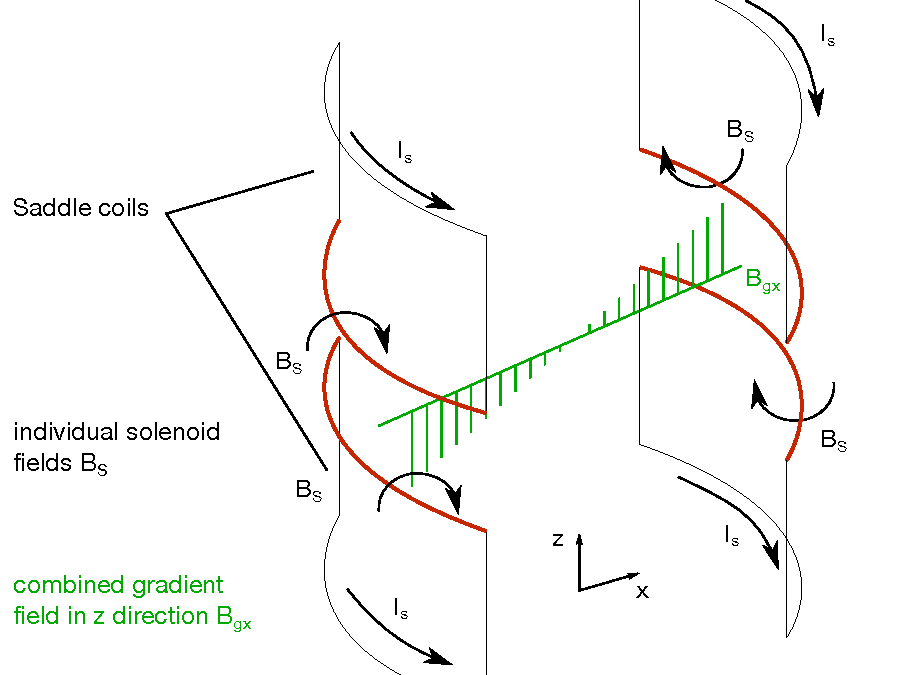
\includegraphics[width=0.99\textwidth]{/figures/materialsMethods/15NSetup/saddleCoilsShim.pdf}
            \caption[Shim coil design]{The design of the shim coils used in the setup. Note that for the x- and y- shims, a design mountable to the PVC tube had to be used in contrast to the z-shims simple maxwell coil design. The field components $B_x$ and $B_y$ mostly cancel out in the relevant volume and $B_z$ follows a mostly linear path if the distances between the pairs are adapted to the PVC tube's radius.}
        \end{figure}
        \subsection{Low field reactor}
        At low field, multiple design features have to be combined to achieve high polarization yields.  First off, ph2 has to be supplied to the sample continuously and efficiently. Positioning of the probe has to be reproducible to ensure the fields are well defined.  The system must be resistant to the chemicals and solvents used in the experiments and hold the pressures applied during measurements.  Furthermore, it must be non magnetic to not distort residual fields inside the shield which otherwise might reduce polarization in parts of the sample. To fulfill all these requirements, polysulphone (psu) was chosen as a material because of its high mechanical and chemical stability.  The reactor was designed in Inventor 2018, Autodesk as a body of rotation. It features a sample volume of about $\SI{3}{\mm\cubed}$ with a larger diameter venting area to reduce sample losses due to foaming and spray as shown in \ref{figure:materialsMethods:probesPSU}, (a3), see indicated diameters. Below the sample volume, a interchangable punched disk ((a3), 2) is installed that provides ph2 to the sample in fine bubbles. By changing the number and diameter of the holes, flow rate and bubble sizes can be adapted to provide ph2 effectively to different kinds of samples and under different conditions.The disk can also be completely removed if only one o ring is inserted instead of the usual two. In case of sample transfer, the conical bottom collects the sample for an efficient and complete sample extraction.  two lines connect to the bottom: one to supply ph2 gas and the other to transfer the sample towards the high field.  An additional gas line connects to the top of the venting area for both de- and pressurization of the sample chamber.
        For dimensinons, see appendix \ref{}
            \begin{figure}
                \centering
                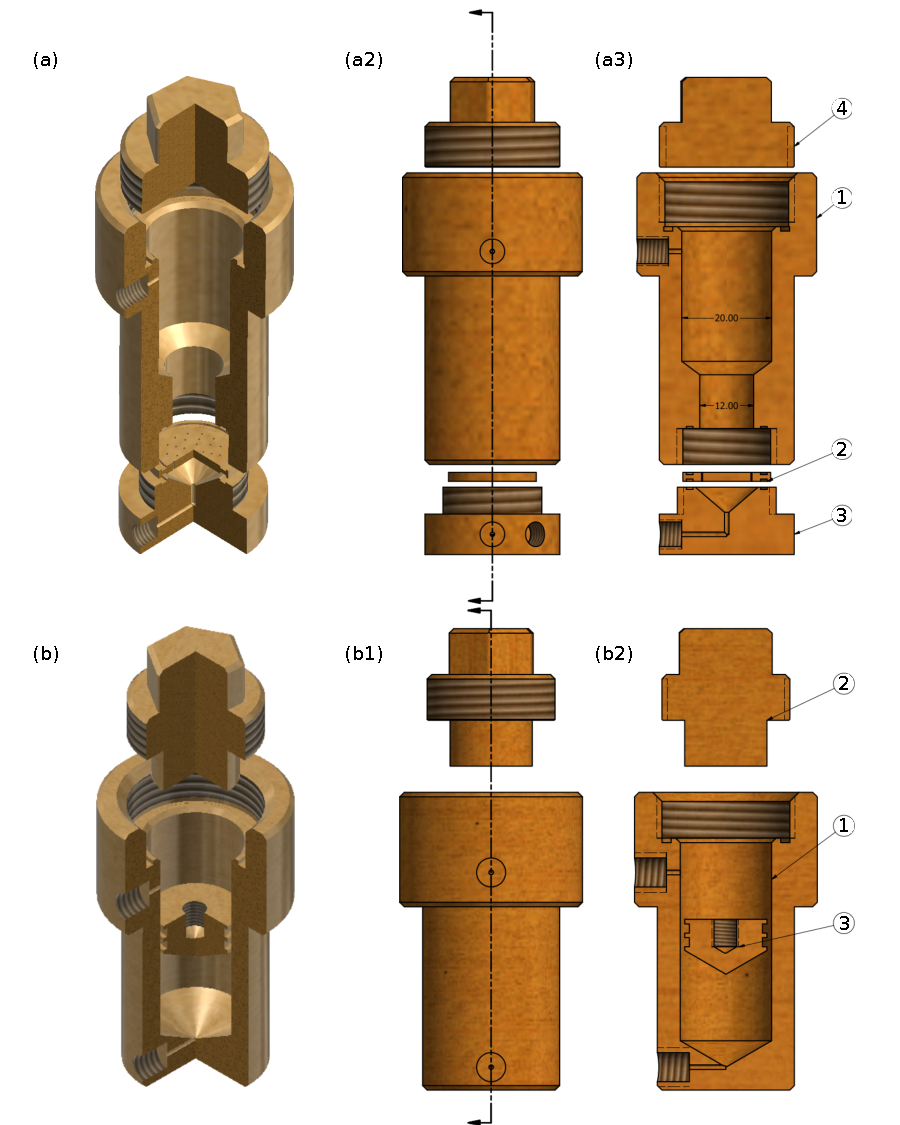
\includegraphics[width=0.99\textwidth]{/figures/materialsMethods/15NSetup/probesPSU.pdf}
                \caption[Reactor gemometry]{Three quarter section views of the low field reactor (top) and high field probe container (end). The disk for ph2 provision in the low field reactor is visisble on the bottom (a3),2 sandwiched between the main body (a3),1 and the screw on cap (a3),3.  Hose connections are made to that cap and the top of the main body. The high field probe (b2),1 is shown with its optional piston inserted (b2),3, the two possible connections at the top for actuation and bottom for sample transfer are visible in the cut views. Both pressure containers are screwed shut wit a lid (a3), 4 and (b3), 2. Seal rings are not shown here.}
                \label{figure:materialsMethods:probesPSU}
            \end{figure}
        \subsection{High field probe container}
        Similarly to the one in low field, the high field probe has to withstand the high pressures applied and the chemicals used. It is made from the same material, PSU.  While its conical bottom is similar to the low field probe's, there's no need for a bubbling system.  Therefore, the body is made of a single part without the possibility of inserting a bubbling disk (see figure \ref{figure:materialsMethods:probesPSU}, (b2), 1).  Once the solution is transferred to the high field probe container, there are two procedures for shuttling the solution back to low field: via a piston hovering above the fluid (fig. \ref{figure:materialsMethods:probesPSU}, (b2), 3) splitting the system into a fluid and a gas side that can be actuated by pressurized gas or simply by the gas pressure that builds above the solution due to the transfer towards high field.  With methanol solutions, the latter method turns out to be efficient, other solutions with different viscosities may need the piston approach for efficient transport.
        For dimensinons, see appendix \ref{}
        \subsection{Fluid handling system}
        The items described above were integrated into a fluid handling system. The whole system is connected by PTFE tubing  using ferrule connections. The tubing has \SI{1/8}{\in} outer and \SI{1/16}{\in} inner diameter for the gas lines and \SI{1/16}{\in} outer and \SI{1/32}{\in} inner diameter PTFE capillary as the fluid connection. The pH2 supply line for the low field reactor is fitted with a check valve mounted as close to the reactor as possible to prohibit the sample from travelling into the supply line.
            \begin{figure}
                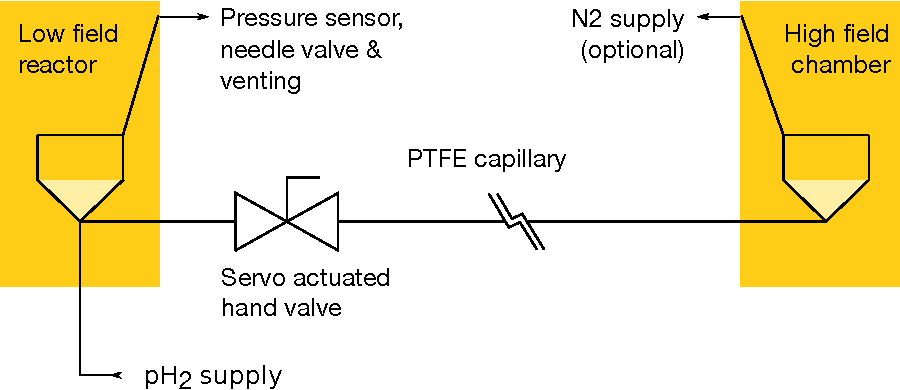
\includegraphics[width=0.99\textwidth]{/figures/materialsMethods/15NSetup/reactorsScheme.pdf}
                \caption[Reactor schematics]{The schematic of the two PTFE reactors on low field side (left) and high field side (right). The connection between both is made by a PTFE capillary separated by the auotmatically actuated hand valve . }
            \end{figure}
            Sample volumes range in the $\SI{3}{\milli\litre}$ regime which means that within the rather large distances of a few meters between high and low field and reactor volumes above sample volumes to enable bubbling, close attention had to be paid to keep fluid losses as small as possible.  The choice of components therefore was focused on low volume parts.  For example, the solenoid valves used for gas supply were not an option for the fluid pathway as the internal volume was so large that different amounts of fluid remained inside the valve making reproducible measurements impossible.  The valve in the fluid transfer path was therefore chosen to be a handvalve of very small intrinsic volume ($\approx$\SI{0.05}{\ml}). The handvalve opens the same way for both sample transport directions with a different pressure gradient between high and low field side. To still be able to automate switching of the valve, a high torque servo motor (MG996R, Tower Pro) has been connected to the valve providing up to \SI{1.1}{\newton\m} torque and serving as electrically steerable actuator. That way, the fluid path consists solely of capillary of \SI{0.18}{\mm} diameter and said hand valve. The other connections are established using \SI{1/8}{in} OD PTFE tubing.  The connections made are:
            \begin{itemize}
                \setlength{\itemsep}{-2pt}
                \item Low field chamber pressurization line
                \item Low field venting line
                \item Low field ph2 supply line
                \item Needle valve outlet for bubbling
                \item Capillary connection for fluid transfer - low to high field
                \item Optional connection: high field nitrogen line for reverse transfer
            \end{itemize}
            \begin{figure}
                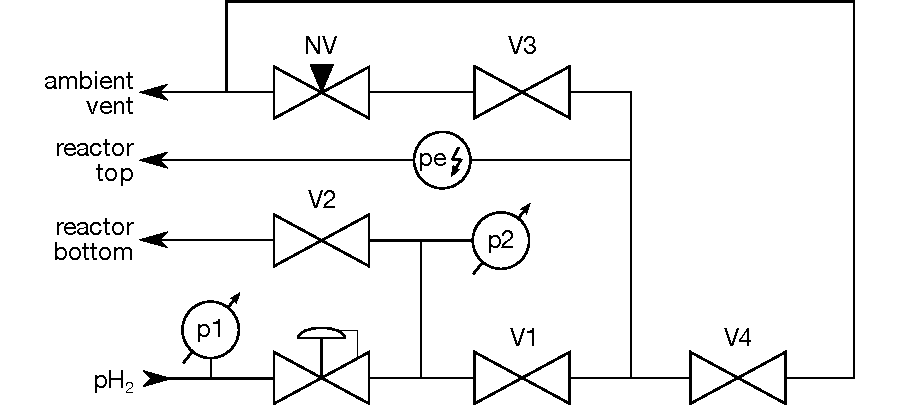
\includegraphics[width=0.99\textwidth]{/figures/materialsMethods/15NSetup/valves15N.pdf}
                \caption[Valve assembly shuttling system]{Schematic view of the valves controlled by the relay box in the shuttling setup. pH2 pressure is regulated and it is distributed to the different stages of the setup. The valves labeled V1 to V4 are solenoid valves. The pressure regulator is not electronically controlled. p1 and p2 are analog pressure sensrors for setting up experiment pressure and monitoring bottle pressure, respectively. 'pe' is an electronic pressure sensor which's reading is fed to tthe microcontroller. Two additional valves to control the floating piston of the high field probe container can be added to the setup.}
                \label{fig:materialsMethods:valveSetup}
            \end{figure}
            Figure \ref{fig:materialsMethods:valveSetup} shows a schematic of the valves used in the fluid handling system. Parahydrogen supplied to the system is first pressure regulated and can then be routed to the different parts of the setup to admit pressure to the reactor from the top (V1), bubble pH2 trough the solution (V2 and V3) or transfer the sample to the high field side (V1 and Handvalve). The other valves are used to depressurize the reactor (V4), transfer the sample back to low field and vent the complete system (V1-V4). The electronic pressure sensor (indicated by the flash symbol, DRTR-AL-20MA-R60, B+B sensors) can be used to reduce pressure to a defined value on the low field side.
            A standard fluid hyperpolarization cycle would consist of: pressurization of the low field chamber to reduce flow when opening the bubbling line.  Opening the bubbling line with a certain pressure and needle valve setting for a certain time.  Closing all valves and opening the transfer line. - the sample is shuttled to high field, the scanner is triggered. - depressurizing the low field chamber (optionally only up to a certain pressure using the pressure sensor).  Reopening the transfer valve to have the sample flow shuttle back to low field (optionally supported by building pressure above the high field floating piston).
            This cycle can be repaeted infinitly, limited of course by the fluid losses through bubbling and the flow towards ambient air and the overall stability of the catalyst in solution. 
            To perform these cycles in a reprducible manner, an automated system has been built controlling as much of the fluid handling system as possible.
        \subsection{Automatic shuttling system}
        To handle the probes in a reprodicible manner and to produce reliable results, a system had to be designed that kept all timings and other parameters under control. A microcontroller was chosen that can be operated independent of other PCs or scanners and is quite flexible that way, i.e. can be adapted to perform different tasks.
        The system connects to the fluid handling system and provides it with gas pressure for fluid transport as well as gas for hyperpolarization, pH2. The system is built mostly from copper tubing (except for the low pressure vent lines). Connections are made via brass ferrule fittings and metal seals. The choise of materials provided long term stability of the system. Te solenoid valves chosen were 2/2 way valves (A5241/1002/.023, GSR Ventiltechnik) of which only four were necessary for basic operation. They can handle pressures up to \SI{85}{\bar} and are operated by \SI{230}{\volt} AC. These valves were supposed to be automatically actuated.
        To do so, a relay card (Relay ISO9002, Songle Relay) was connected to all the valves to handle switching with a microcontroller. The relay can handle currents up to \SI{7}{\ampere} at voltages up to \SI{240}{\volt} AC (or \SI{10}{\ampere}, \SI{28}{\volt} DC) for resistive loads. The automation concerned the solenoid valves (that were previously actuatet by flipping a switch), but also the automated handvalve and its servo motor. The microcontroller of choice was, as in many cases in this work, a teensy 3.6 (PJRC, 3.3v). All components were installed inside a box (relay box) that featured eight female IEC sockets enabling a safe operation of the \SI{230}{\volt} valve supply voltage.  Internally, eight digital outputs of the teensy were connected to the relaycard.  For galvanic isolation, a optocoupled design was chosen (see figure \ref{fig:materialsMethods:relaySchematics} for details).
        \begin{wrapfigure}{r}{0.5\textwidth}
                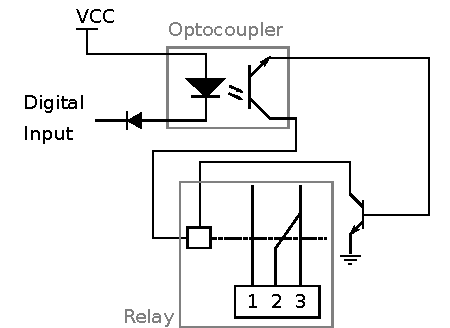
\includegraphics{/figures/materialsMethods/15NSetup/optoRelayScheme.pdf}
                \caption[Relay schematics]{One relay module of which 8 were mounted onto a single PCB board in this case. Note the galvanic isolation through the optocoupler in the top center of the schematics.}
                \label{fig:materialsMethods:relaySchematics}
            \end{wrapfigure}
            The relay board and the teensy were supplied by a \SI{230}{\volt} AC powered \SI{5}{\volt} DC power supply.  To execute valve sequences, eight buttons were installed in the cover of the box.  Additionally, eight switches were added.  That way, depending on the program run on the teensy, switches and buttons can control either single valves directly or execute valve sequences for shuttling sample into and out of the scanner.
            \begin{table}
                \centering
                \begin{tabular}{| l | c | cccc | ccc | r |}
                    \hline
                    Step & \rotatebox{90}{Duration} & \rotatebox{90}{V1} & \rotatebox{90}{V2} & \rotatebox{90}{V3} & \rotatebox{90}{V4} & \rotatebox{90}{Handvalve open} & \rotatebox{90}{Scanner trigger} & \rotatebox{90}{Pressure sensor} & \rotatebox{90}{Comment}\\
                    \hline
                                                % 1 & 2 & 3 & 4 & HV& ST& PS& comment
                    Activation  & \SI{1}{\s}    & x & - & - & - & - & - & - & build pressure \\
                                & \SI{20}{\min} & - & x & - & - & - & - & - & bubble for activation \\
                    \hline
\tikzmark{repBeg}    Bubbling  &\SI{20}{\s}     & - & x & - & - & x & - & - & hyperpolarize sample \\
                    \hline
                    Transfer in  &\SI{3}{\s}     & x & - & - & - & x & - & - & fluid flow \\
                                &\SI{0.5}{\s}   & - & - & - & - & - & - & - & close handvalve\\
                    \hline
                    Trigger scan&\SI{0.1}{\s}   & - & - & - & - & - & x & - & trigger module on \\
                    \hline
                  Transfer out&\SI{0.1}{\s}     & - & - & - & x & - & - & - & release pressure \tikzmark{release}\\
                            &\SI{10}{\milli\s}     & - & - & - & - & - & - & x & optional pressure read \tikzmark{pr}\\
                                &\SI{3}{\s}     & - & - & - & - & x & - & - & fluid flow \\
                    \hline
\tikzmark{repEnd}   Prepare bubbling&\SI{1}{\s} & x & - & - & - & - & - & - & build pressure again\\
                    \hline 
                \end{tabular}
                \begin{tikzpicture}[overlay, remember picture]
                    \begin{scope}[c/.style={shift={(\tabcolsep, \the\dimexpr\fontdimen12\textfont2\relax)}}]
                        \draw[->] ([c]pic cs:release) to [bend left] node[right] {feedback loop}([c]pic cs:pr);
                        \draw[->]  ([c]pic cs:pr) to [bend left]([c]pic cs:release);
                    \end{scope}
                    \begin{scope}[c/.style={shift={(-\tabcolsep, \the\dimexpr\fontdimen12\textfont2\relax)}}]
                        \draw[->] ([c]pic cs:repBeg) -- +(-.2,0) to [bend right=1] ([c, shift={(-0.2,0)}]pic cs:repEnd) -- ([c]pic cs:repEnd);
                        \draw[->] ([c]pic cs:repEnd) to [bend left=140] node[left]{$\cdot$ n}([c]pic cs:repBeg);
                    \end{scope}
                \end{tikzpicture}
                \caption[15N hyperpolarization steps]{A standard shuttling circuit as used in most of the experiments. The activation step is performed once per sample. The shuttling procedure can be repeated as often as necessary as long as the sample is still working and fluid losses are within bounds. The pressure release can optionally be performed up to a certain pressure value only.}
            \end{table}
            In addition to the solenoid valve sockets, two low voltage parallel ports were installed.  They were used to control the servo motor of the automated hand valve and to read out the pressure sensor of the setup.  More sensors or controllers can easily be added as about $\frac{3}{4}$ of the parallel port pins are still blank.
            a last outgoing connection was a coaxial jack for scanner triggering.  As described in the results section, hf-feedback from the relay made a two staged low-pass frequency filter necessary to prevent accidental scanner triggering.
    \section{Magnetic fluxgate field probe}\label{sec:methodsfluxgate}
        To measure fields very precisely, the most common hall sensor mehtod is not sensible enough. Therefore other principles such as Squids or fluxgates have to be used at very low fields. In our case, a three-axis fluxgate was purchased.
        \subsection{Measurement principle}
            The measurement principle behind a fluxgate is based on the hysteresis of magnetic materials. To make use of the hysteresis effect, a ferromagnetic material is continuously polarized in alternating directions. The voltage and current throughout the hysteresis are measured. If an external field is applied to the material, this will shift the hysteresis curve as a larger field will be necessary to saturate the material in the direction countering the external field and a smaller field in the direction parallel to the external field (or its component(s)). This shift can be measured electronically and will provide very precise information about the external field causing the shift and can be used to measure fields in the \si{\nano\tesla} range.
        \subsection{Power supply}
            As the fluxgate needed a power supply of $\pm$ \SI{15}{\volt} that was not provided with the sensor, a DC \SI{24}{\volt} power suply was fitted with a high efficiency $\pm$ \SI{15}{\volt} DC-DC-converter (PDM1-S24-D15, CUI INC). It features short circuit protection as well as a protection against static discharge of up to \SI{8}{\kilo\volt}. The DC-DC-converter was fitted into the power supply's casing. The original cable was replaced by a three-wire.
        \subsection{Arduino uno shield}
            As a first test, a shield for a 12 bit arduino microcontroller was built reading out the individual channels on individual analog inputs.  Depending on the output voltage, the signal was fed to the analog input unpertubated or split throug a voltage divider if it rose above the analog inputs maximum voltage.  The shield was etched in a \todo{acid?} bath after uv-exposure of the light sensitive pcb and development in a \todo{bath}.  For exposure, a printed foil bag has been used into which the two sided pcb was inserted  its sides were uv-exposed individually.  As the resolution of this design was not sufficient for the low fields generated inside the mu metal shield, it had to be discarded for a solution featuring active amplification.
        \subsection{Teensy 3.6 shield}
            The alternative solution using a teensy 3.6 microcontroller (PJRC, \SI{3.3}{\volt}) and a self designed shield provided higher intrinsic bit depth and additional active amplification using operational amplifiers.  The board was designed using eagle CAD as before using the autorouting function once the components were placed on the PCB virtually.  In most cases, the traces did not need correction, but some small details were changed e.g.  To keep supply leads of the individual components short or to keep signal leads away from rf-influences.  The overall size of the board was \SI{64}{\mm} x \SI{54}{\mm}.  Top and bottom layer were connected through 66 vias, no intermediate layers were required.  The leads width was chosen to be \SI{10}{mil} (\SI{0.254}{\mm}) for both signal and power supply leads as it was deemed enough for the currents necessary. 
            Amplification was performed in two steps, all operational amplifiers were contained in a single smd-part though (MAX44245-SO14, Maxim Integrated). Analogue switches (ADG1402, Analog Devices) were mounted for each Op-Amp, i.e. each amplification and for each channel individually. The amplifications were chosen to be 1, 4 and 16 for each of the amplification stages. The total amplification range from 1 to 256 accordingly. A precision \SI{3}{\volt} voltage reference was installed (ADR423, Analog Devices) for low noise, high precision measurements adjustable via a rotatable resistor. As a power supply, a step down (LM2675, Texas Instruments) that was fed by the $\pm$\SI{15}{\volt} dc-dc-converter of the fluxgate itself. To reduce RF-influences, a low-pass filter was fit to the data line before the analog input of the teensy. 
            \begin{figure}
                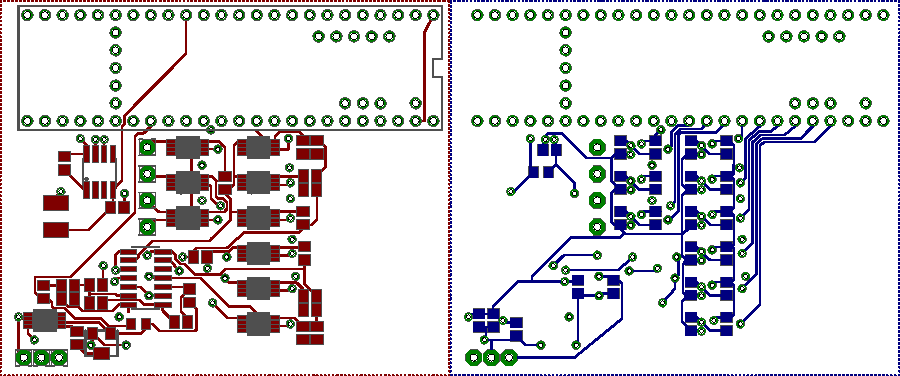
\includegraphics[width=0.99\textwidth]{/figures/materialsMethods/15NSetup/boardTopAndBottom.pdf}
                \caption[Fluxgate board layout]{The board layout of the fluxgate electronics as designed in eagle CAD. On the left, in red, the front with all the main components, i.e. ICs mounted to its surface. On the right, in blue, the back side with the supply voltage capacitors opposite of each IC. The top left three analog switches are for changing the channel, the tree next to them constitute the first amplification stage. Below is the second amplification stage that is finally read out by the teensy indicated on top.}
                \label{fig:materialsMethods:fluxgateBoard}
            \end{figure}
        \subsection{Teensy programming}
        Programs were uploaded to the microcontroller via a standard micro usb cable using the arduino software environment. I recommend using external editors such as vim or emacs as the internal text editing functions of the arduino environment are quide rudimentary. The program runnning on the teensy microcontroller reads out the three channels of the fluxgate serially with a delay of \ref{}. This delay was added manually to prevent switching artifacts. Each individual channel receives an amplification that is automatically adapted on the fly. Magnetic fields are calculated from the measured values using bit depth and amplification. All sensors' individual readings, the corresponding magnetic fields and the calculated total magnetic field are displayed on a simple 160x128 pixel display (1.8" mini serial SPI, IC ST7735B) driven by the adafruit libraries (Adafruit\_ST7735.h). Note that, due to the different voltage levels of teensy and display, either a \SI{3.3}{\volt} to \SI{5}{\volt} bidirectional converter needs to be used or \SI{10}{\kilo\ohm} resistors need to be added to the data lines of the display. In addition to the final software version, several testing programs have been written: A "boardTest" program that switches the amplifications in a predefined manner to test analogue switches, a "testAmplifications" program that switches amplifications to test those and the operational amplifiers and a tftTest program to see whether the display is connected properly and displays the expected data due to initial problems with the tft libraries. All the testing programs use the serial I/O of the microcontroller to display data, a usb serial connection is necessary to use the full range of features.
        \subsection{Cabling and boxing}
        The complete assembly of power supply cable, teensy, display and Fluxgate cable were fitted into a box with the display showing on top and connected internally \ref{figure cabling}. A hole to reprogram the microcontroller without opening the box was added. Note that when plugging in the power supply, it has to be connected to the box. Otherwise, the teensy will not boot properly.
%\input{}
